% Created 2017-01-22 Sun 14:04
% Intended LaTeX compiler: pdflatex
\documentclass{scrartcl}
\usepackage[utf8]{inputenc}
\usepackage[T1]{fontenc}
\usepackage{graphicx}
\usepackage{grffile}
\usepackage{longtable}
\usepackage{wrapfig}
\usepackage{rotating}
\usepackage[normalem]{ulem}
\usepackage{amsmath}
\usepackage{textcomp}
\usepackage{amssymb}
\usepackage{capt-of}
\usepackage{hyperref}
                \usepackage[newfloat]{minted}
\usepackage[hypcap=false]{caption}
                \usepackage[left=2cm,right=2cm,top=1.5cm,bottom=1.5cm,marginpar=0cm, includeall]{geometry}
\usepackage{lmodern}
\usepackage[germanb]{babel}
\usepackage{eurosym}
\setlength{\parindent}{0pt}
\usepackage{blindtext,lastpage,scrpage2}
\usepackage{fancyhdr}
\pagestyle{scrheadings}
\chead{Thomas Fragner (1455954), Sandra Pühringer (1456472)}
\cfoot{\thepage{} von \pageref{LastPage}}
\RequirePackage{fancyvrb}
\DefineVerbatimEnvironment{verbatim}{Verbatim}{fontsize=\scriptsize}
\author{Thomas Fragner (1455954), Sandra Pühringer (1456472)}
\date{\today}
\title{Communications Engineering UE\\\medskip
\large CEBay Seeder und Client - Vorgehen}
\hypersetup{
 pdfauthor={Thomas Fragner (1455954), Sandra Pühringer (1456472)},
 pdftitle={Communications Engineering UE},
 pdfkeywords={},
 pdfsubject={},
 pdfcreator={Emacs 25.1.1 (Org mode 9.0.1)}, 
 pdflang={Germanb}}
\begin{document}

\maketitle
\tableofcontents

\newpage
\section{Server (Seeder)}
\label{sec:orgc9e2986}
Der Server stellt Daten bereit. Diese registriert der Server am
Registry Server der CEBay. Der Server ist aus mehreren Komponenten
zusammengestellt:
\begin{description}
\item[{ServerApp}] ist die eigentliche Application. Sie dient als Command
Line Frontend für den Server. Das Actor System wird von der
ServerApp erstellt. Weiters startet die Application enen Actor
vom Typ ActorSeederManager.
\item[{ActorSeederManager}] Dieser Actor verwaltet die bereitzustellenden
Dateien und erstellt für jede Datei einen Actor ActorSeeder.
\item[{ActorSeeder}] Bearbeitet Downloadanfragen für eine Datei
\end{description}

\begin{center}
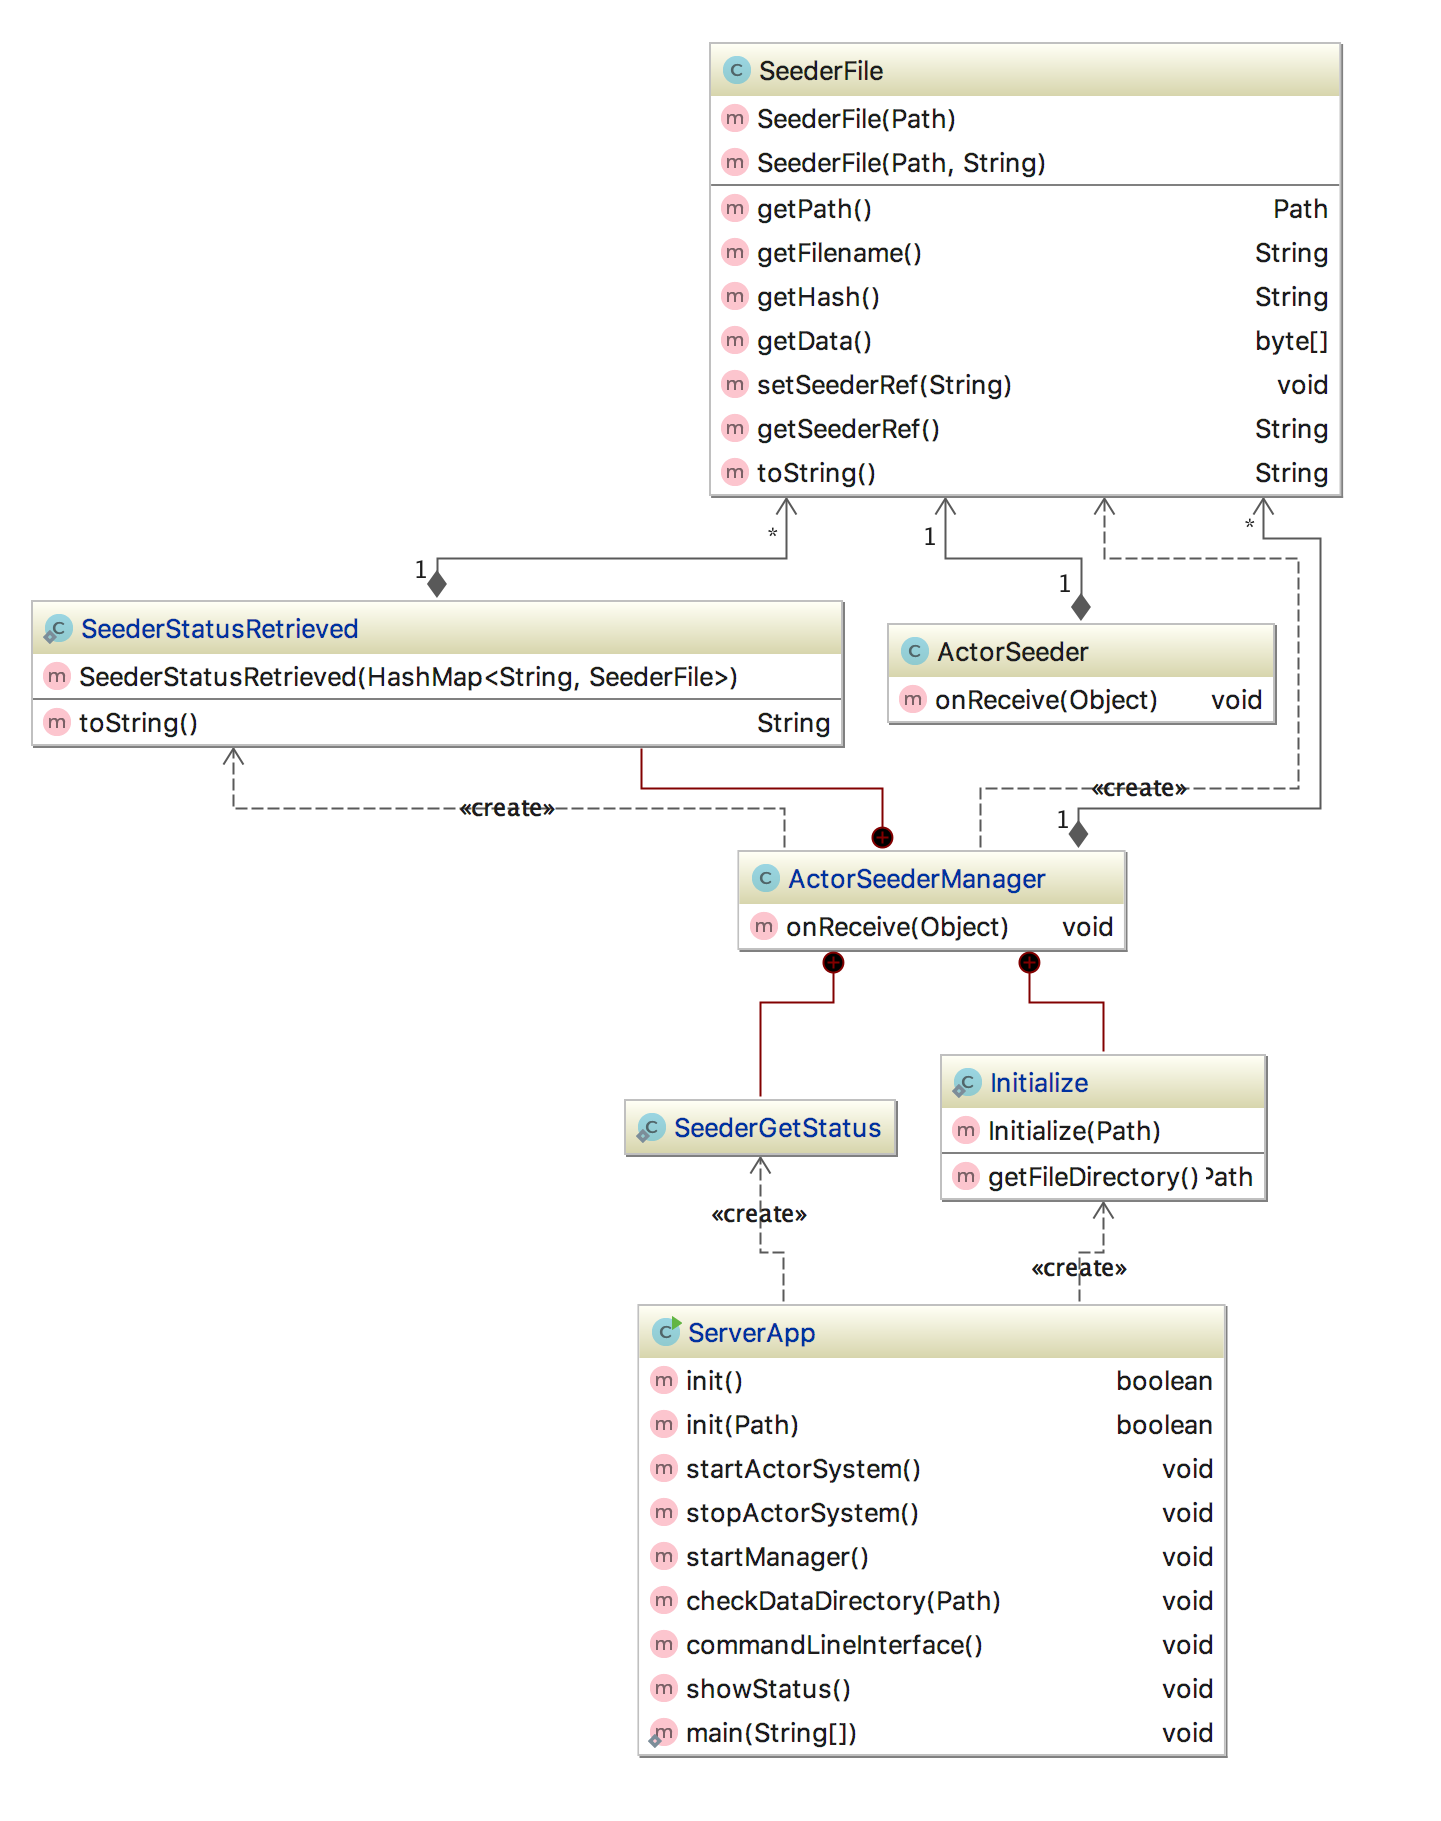
\includegraphics[width=.7\textwidth]{diagram_server.png}
\captionof{figure}{Klassenstruktur Server}
\end{center}

\subsection{ServerApp}
\label{sec:org991ff42}
Die Klasse ServerApp stellt einen ausführbares Programm zur
Verfügung. Beim Starten erzeugt es ein Actorsystem und startet einen
Actor ActorSeederManager. Diesem Actor kann beim Erstellen ein Pfad zu
einem Verzeichnis übergeben werden, in dem die bereitzustellenden
Dateien gesucht werden. Nach dem Start des Actors wird ein Command
Line Interface angeboten. Dieses bietet die Möglichkeit eine
Statusabfrage zu allen bereitgestellen Dateien abzurufen.

\subsection{ActorSeederManager}
\label{sec:org18483df}
Die Klasse ActorSeederManager stellt einen Actor zur Verfügung. Dieser
Actor verwaltet alle bereitzustellenden Dateien. Der Actor bearbeitet
die folgenden Nachrichten:

\begin{description}
\item[{Initialize}] Mit dieser Nachricht wird der Manager
initialisiert. In der Nachricht ist der Pfad zum Verzeichnis mit
den bereitzustellenden Dateien enthalten. Im Zuge der
Initialisierung werden alle Dateien die sich in diesem
Verzeichnis befinden bei der CEBay Registry registriert. Für jede
gefundene Datei sendet der Actor eine Nachricht vom Typ SeederFile an
sich selbst.
\item[{SeederFile}] Wenn eine Nachricht vom Typ SeederFile erhalten wird,
dann erzeugt der Actor einen neuen Kind-Actor vom Typ
ActorSeeder. Die Instanz von SeederFile wird um die ActorRef des
erstellten Actors erweitert. Anschließend wird diese Instanz von
SeederFile an den neuen Actor gesendet. Zusätzlich wird die
Erstellung des neuen Aktors in einer HashMap gepseichert.
\item[{SeederGetStatus}] Beim Eintreffen dieser Nachricht wird die HashMap
mit den Status der bereitgestellten Dateien in Form einer
Nachricht vom Typ SeederStatusRetrieved an den Sender zurückgesendet.
\item[{UploadFile}] Diese Nachricht enhält Daten für eine neue Datei. Beim
Erhalt der Nachricht wird das in der Nachricht enthaltene Byte
Array in das Datenverzeichnis gespeichert. Der Dateiname der
neuen Datei ist ebenfalls in der Nachricht enthalten.
\end{description}

\subsection{ActorSeeder}
\label{sec:orge4b8ee0}
Die Klasse ActorSeeder stellt den eigentlichen Seeder zur
Verfügung. Hauptaufgaben des Actors sind:
\begin{itemize}
\item die Registrierung an der CEBay
\item Downloadanfragen bearbeiten
\item Statusabfragen beantworten
\end{itemize}

Folgende Nachrichten werden von Actor bearbeitet:
\begin{description}
\item[{SeederFile}] Beim Erhalt einer Nachricht vom Typ SeederFile wird
die entsprechende Dateie bei der CEBay registriert. Dabei wird
eine Nachricht vom Typ Publish mit dem Dateinamen, dem Hashwert
der Datei und der ActorRef als String gesendet.
\item[{GetFile}] Bei einer Nachricht des Typs GetFile wird die vom Client
angefrage Datei in eine Nachricht vom Typ FileRetrieved
verpackt. und an den Sender als Antwort zurückgeschickt. Sollte
die angefragte Datei nicht mir der Datei des Actors überenstimmen
wird eine Nachricht FileNotFound gesendet.
\item[{GetStatus}] Bei einer Statusanfrage durch die CEBay oder einen
Client wird eine Nachricht vom Typ StatusRetrieved zurückgesendet.
\end{description}
\newpage
\section{Client}
\label{sec:orgc30708e}

\subsection{ClientApp}
\label{sec:org3cdccec}
Die Klasse ClientApp stellt ein ausführbares Programm zur
Verfügung. Die folgenden Funktionalitäten werden vom Programm
bereitgestellt:
\begin{itemize}
\item Erstellen eines Actor Systems
\item Erstellen des Downloadmanagers
\item Abrufen der Dateiliste von der CEBay
\item Download einer gewählten Datei
\item Download aller verfügbaren Dateien
\item Status der Downloads
\item Upload einer neuen Datei
\end{itemize}

\begin{center}
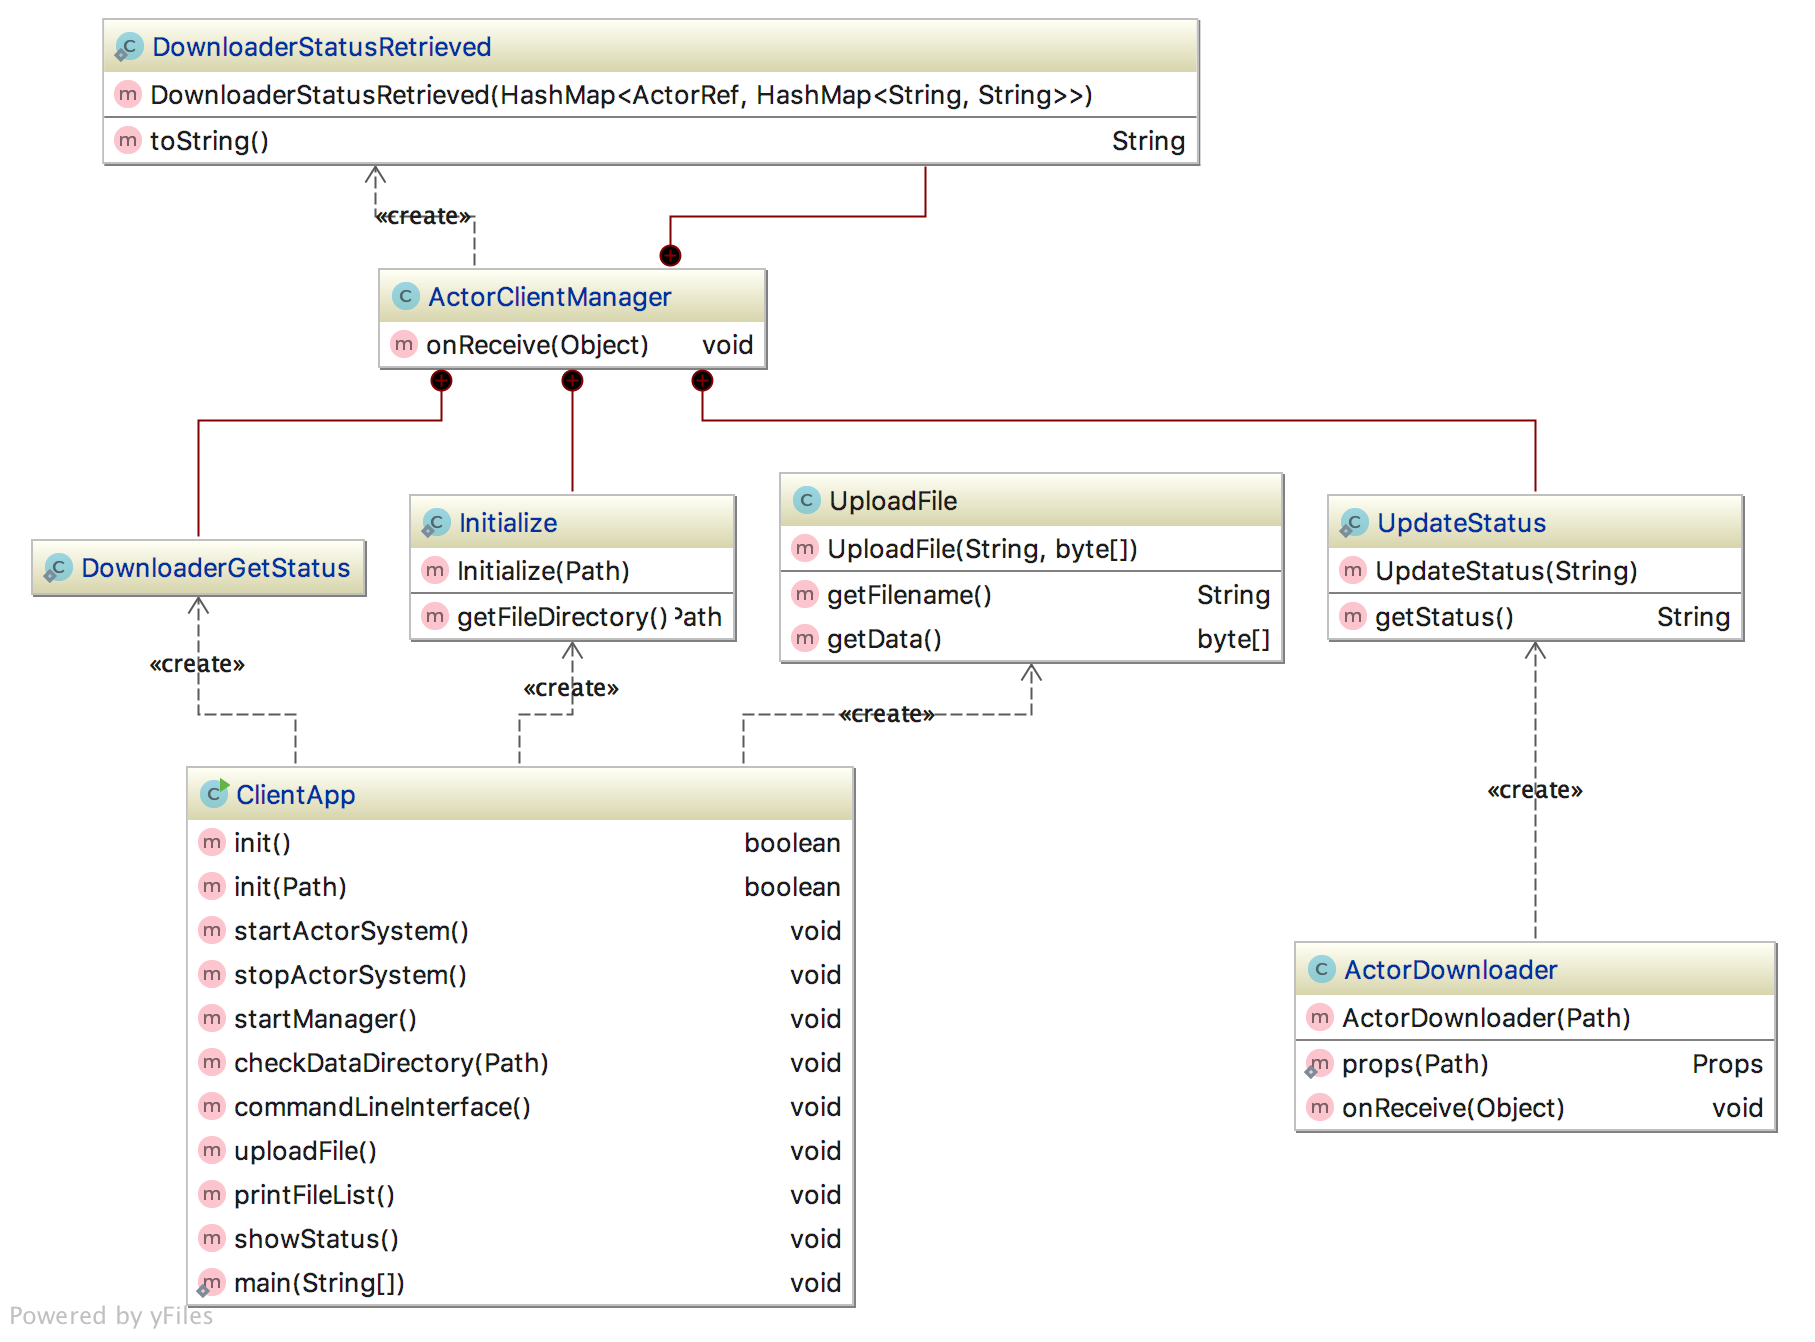
\includegraphics[width=.9\textwidth]{diagram_client.png}
\captionof{figure}{Klassenstruktur Client}
\end{center}

Beim Abrufen der Dateiliste wird eine Nachricht vom Typ GetFileNames
an die CEBay gesendet. Als Antwort kommt eine Liste mit verfügbaren
Dateien zurück. Aus dieser Liste kann der Benutzer eine Datei
auswählen, die heruntergeladen werden soll. Der Dateiname wird
anschließend an den ActorClientManager übergeben. Weiter kann ein
Upload gestartet werden. Dazu wird eine Nachricht vom Typ UploadFile
an einen Seeder gesendet.
\subsection{ActorClientManager}
\label{sec:orgad638f8}
Die Klasse ActorClientManager stellt einen Actor zur Verfügung. Dieser
Actor verwaltet alle Downloads. Der Actor bearbeitet die folgenden
Nachrichten:

\begin{description}
\item[{Initialize}] Das Downloadverzeichnis wird festgelegt.
\item[{GetFile}] Bei einer Anfrage des Client Programms vom Typ GetFile
wird ein neuer Actor vom Typ ActorDownloader erstellt. Die
erhaltene Nachricht wird an diesen Actor weitergeleitet.
\item[{downloaderGetStatus}] Bei Erhalt dieser Nachricht wird der Status
der Downloads zurückgesendet.
\item[{UpdateStatus}] Actor vom Typ ActorDownloader können diese Nachricht
senden um den aktuellen Status bekanntzugeben. Wenn der Status
"failure" ist wird der entsprechende ActorDownloader beendet.
\end{description}
\subsection{ActorDownloader}
\label{sec:orge27889b}
Die Klasse ActorDownloader wickelt genau einen bestimmten Download
ab. Dazu werden folgenden Nachrichten verwendet:
\begin{description}
\item[{GetFile}] Diese Nachricht weist den Actor an eine bestimmte Datei
herunterzuladen. Im ersten Schritt werden die verfügbaren Seeder
für die Datei bei der CEBay nachgefragt.
\item[{SeederFound}] Bei einer Antwort von der CEBay mit einer Nachricht
vom Typ SeederFound wird an alle Seeder eine Nachricht vom Typ
GetStatus gesendet. Damit soll festgestellt werden welche Seeder
tatsächlich verfügbar sind. Es wird eine Antwort vom Typ
StatusRetrieved erwartet.
\item[{StatusRetrieved}] Sobald sich ein möglicher Seeder meldet, werden
keine weiteren Meldung vom Typ StatusRetrieved mehr akzeptiert
und es wird eine Nachricht vom Typ GetFile an den entsprechenden
Seeder gesendet. Weiters wird eine Nachricht an den Download
Manager geschickt, dass der Download begonnen hat.
\item[{FileRetrieved}] Sobald der Seeder eine Nachricht vom Typ
FileRetrieved zurücksendet wird diese Nachricht verarbeitet und
die enthaltene Datei im Downloadverzeichnis abgespeichert. Danach
wird eine Nachricht an den Download Manager gesendet, dass der
Download fertig ist.
\item[{FileNotFound}] Wenn diese Nachricht eintrifft wird eine Meldung an
den Download Manager gesendet um bekanntzugeben, dass der
Download nicht funktioniert.
\end{description}

Weiter gibt es einen internen Timer. Wenn nach 90 Sekunden kein
Seeder gefunden wurde wird ebenfalls ein Fehlschlag an den Download
Manager gemeldet. Dies führt dann zum Beenden des Actors.

\newpage
\section{Sequenz Diagramm}
\label{sec:orga13b454}
\begin{center}
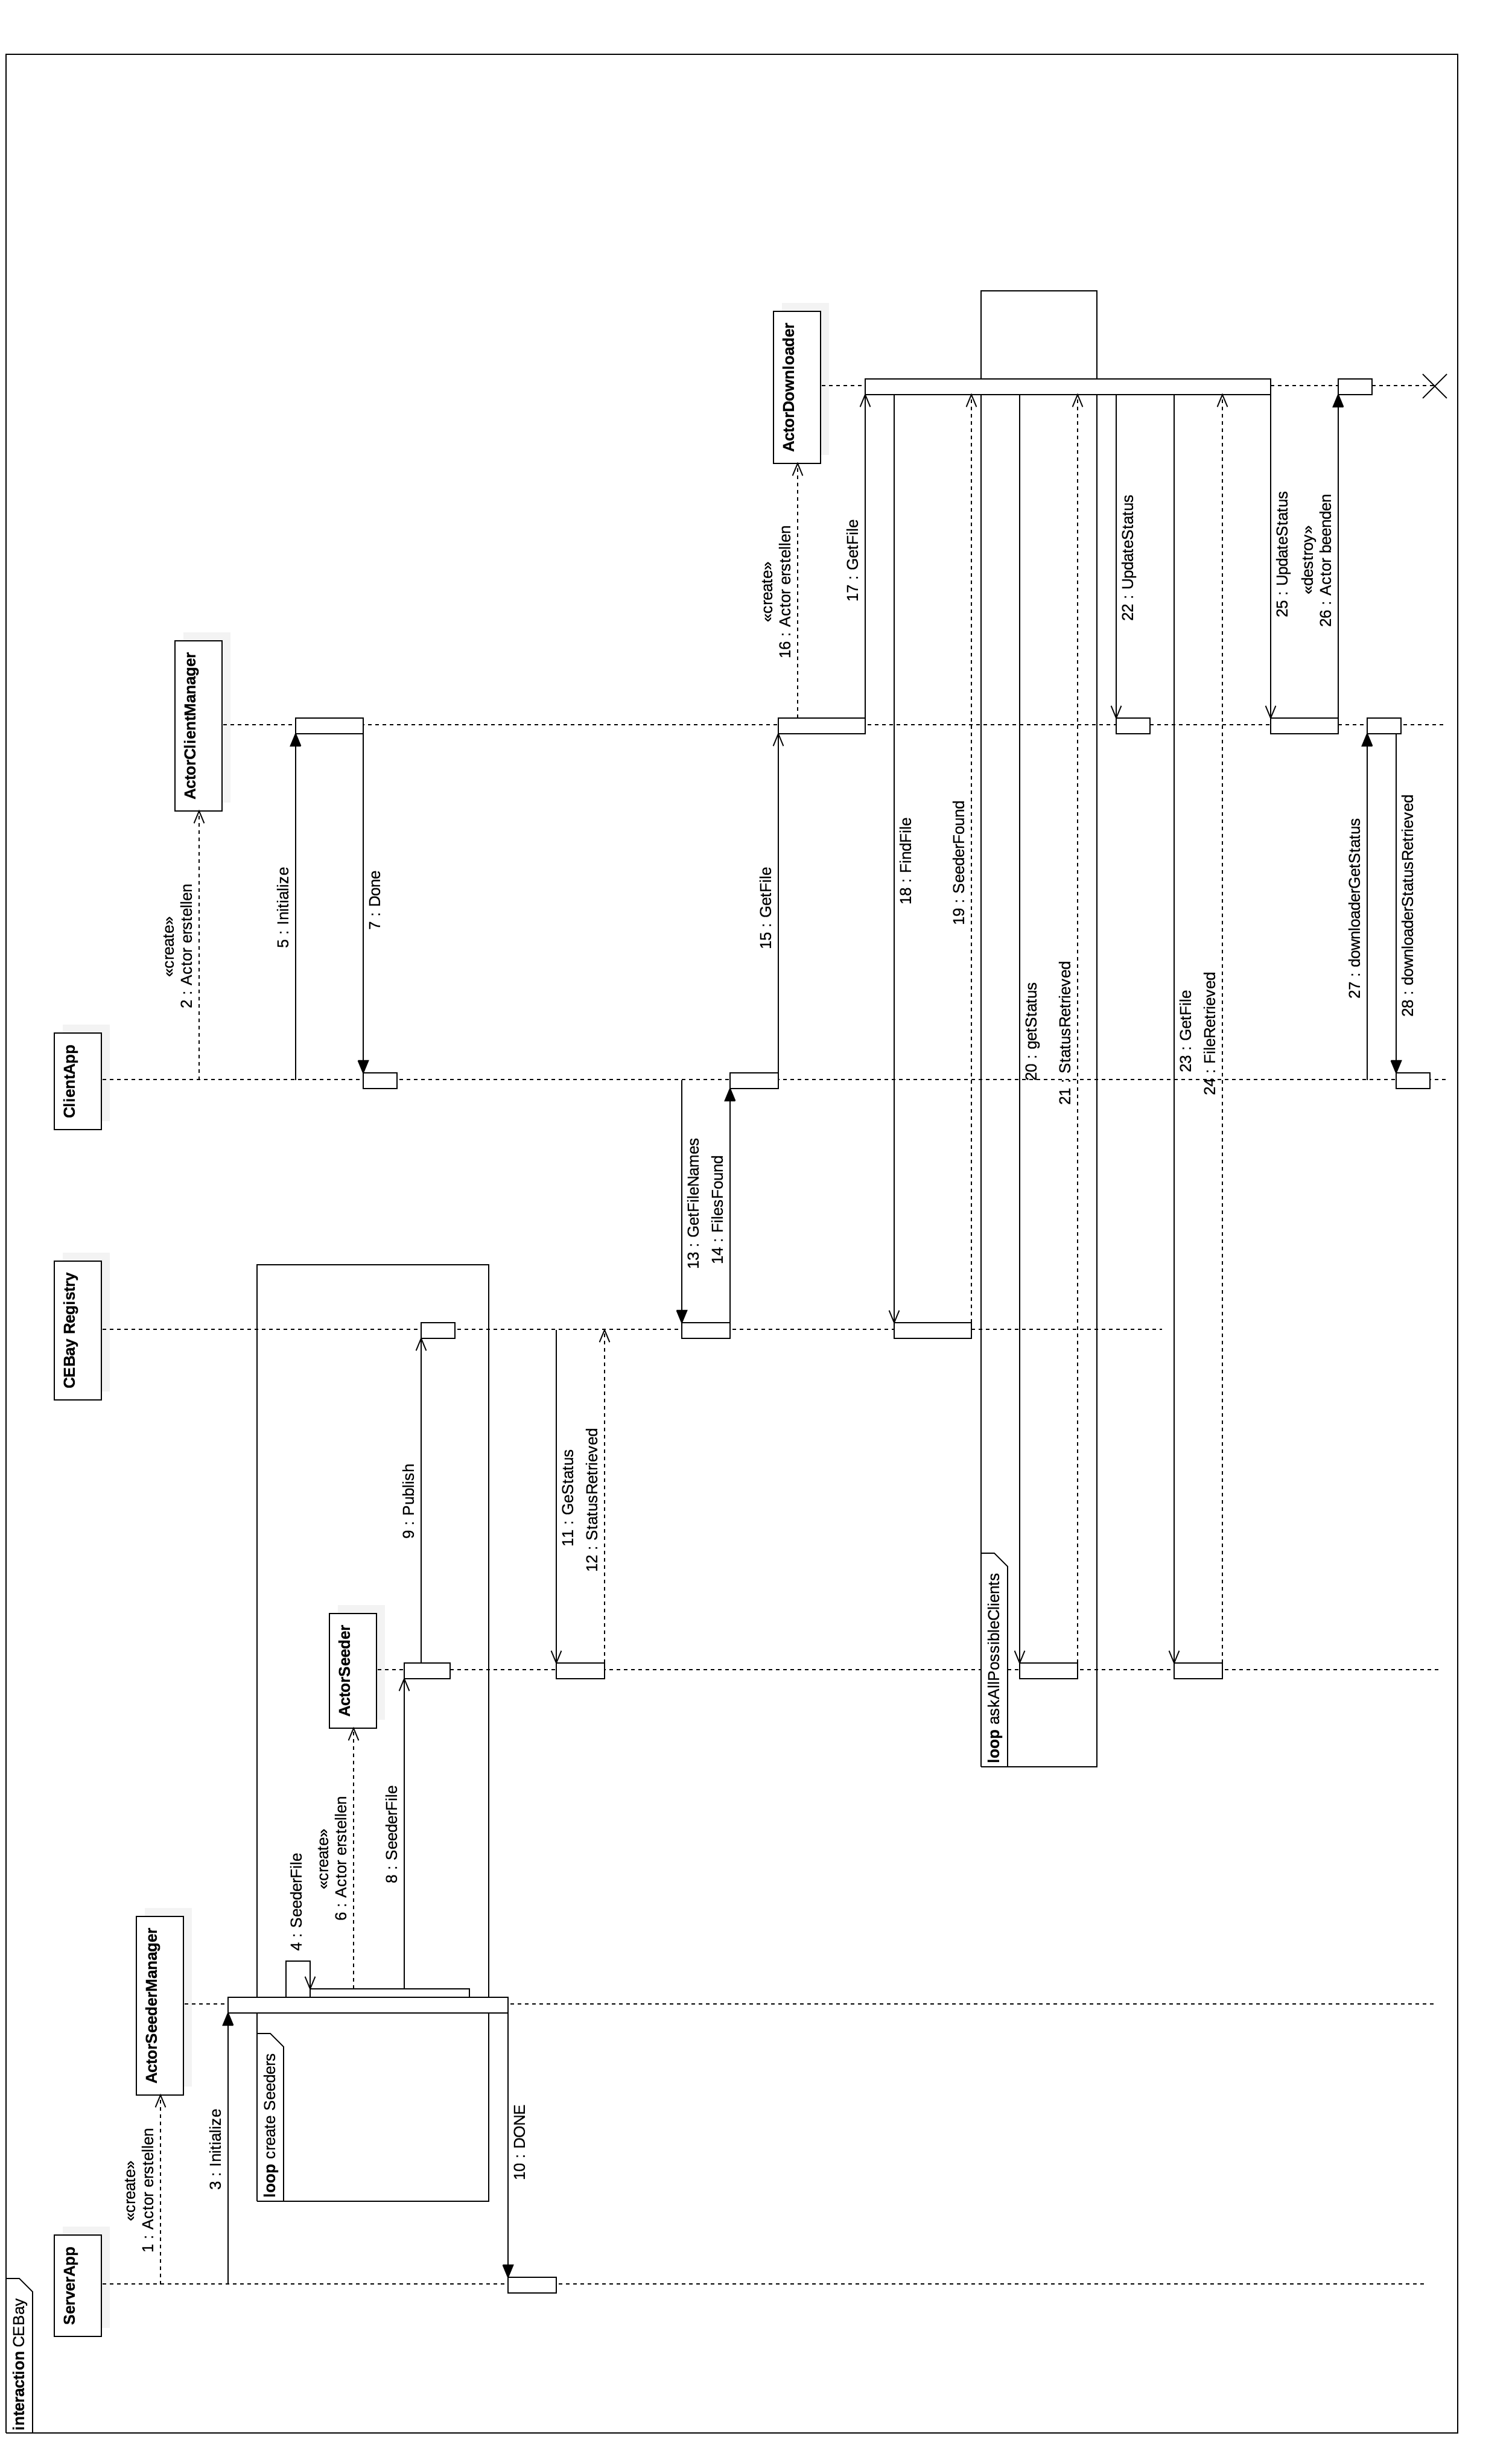
\includegraphics[height=.9\textheight]{sequence_diagram.png}
\captionof{figure}{Sequenz Diagramm}
\end{center}
\end{document}
